\section{Approximating the Pareto-optimal set}

\begin{itemize}
\item [\textbf{2008}] RM-MEDA: A Regularity Model-Based Multiobjective Estimation of Distribution Algorithm~\cite{4358761}
\item [\textbf{2009}] Approximating the Set of Pareto-Optimal Solutions in Both the Decision and Objective Spaces by an Estimation of Distribution Algorithm~\cite{5208353}
\end{itemize}

As in Figure \ref{fig:approximate_pareto_optimal}, the Pareto front is modeled by
\begin{itemize}
\item a Utopian PF(an $(m-1)$-D simplex) in objective space by population $ P $
\item $ K $ - number of subpopulations of $ P $
\item $ Y^{1} \cdots Y^{K} $ as $ K $ reference points uniformly spread on the Utopian PF
\item cluster $ P $ into $ K $ subpopulations $ P^{1} \cdots P^{K} $
\item perform PCA on each $ P^{k} $
\end{itemize}

\begin{figure}
\centering
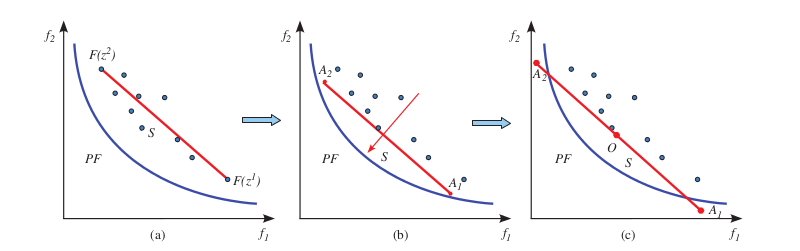
\includegraphics[width=0.7\linewidth]{./img/approximate_pareto_optimal}
\caption{Approximate Pareto-optimal set}
\label{fig:approximate_pareto_optimal}
\end{figure}
